
	Definiamo un altro problema di classificazione che trattiamo questa volta con SVM.
	Il termine di regolarizzazione che possiamo ottimizzare questa volta è il parametro C, tenendo conto che se usiamo valori bassi di C allora la soluzione sarà smooth, mentre se usiamo valori grandi per C ci interessiamo solo a minimizzare l'errore e avremo una soluzione più complicata.
	Per ottimizzare il termine su C cicliamo su di esso per vari valori per trovare il vettore $\alfa$ che più sparso, cioè con il maggior numero di zeri, e il modello w corrsipondente. A questo punto con il valore ottimo di C e il rispettivo modello plottiamo la soluzione.
	We define another classification problem that we deal with this time with SVM.
	The regularization term that we can optimize this time is the C parameter, taking into account that if we use low C values then the solution will be smooth, whereas if we use big C values we are only interested in minimizing the error and will have a more complicated solution .
	To optimize the term on C we cycle on it for various values to find the scattered $ \ alpha $ vector, ie with the greatest number of zeros, and the corresponding w model. At this point with the optimal value of C and the respective model we plot the solution.
	
	\begin{figure}[h]
		\centering
		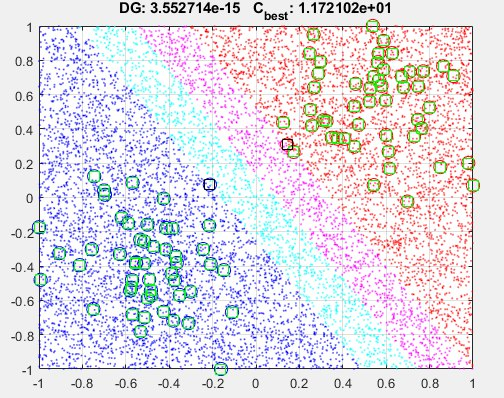
\includegraphics[width=0.5\textwidth]{i2.png}
		\caption{Regression Function}
		\label{fig:regression function}
	\end{figure}
